\section{Corruption Breaks Safety Before Capability}
\label{sec:results}

\subsection{Safety degrades broadly and consistently}
\label{sec:results:main}

\begin{table}[t]
  \centering
  \caption{\textbf{Image corruptions weaken safety.} Final-answer harmful rate HR\textsubscript{C} (\%) on SIUO (167 items, GPT-4o judge); higher = less safe. 16 of 18 model$\times$corruption cells increase (two-sided sign test, $p{=}0.0013$), and every configuration degrades under zoom blur. The two decreases (LlamaV-o1, gray) are not significant under exact McNemar tests on paired per-item verdicts ($p{=}0.56$, $p{=}0.82$).}
  \label{tab:siuo-main}
  \small
  \setlength{\tabcolsep}{4.5pt}
  \begin{tabular}{lccccc}
    \toprule
    Model & clean & glass & snow & zoom & $\Delta$max \\
    \midrule
    Llama-3.2-V (base) & 60.5 & 61.1 & 64.7 & 69.5 & $+9.0$ \\
    LLaVA-CoT          & 68.3 & 71.3 & 71.9 & 74.8 & $+6.6$ \\
    Qwen2.5-VL         & 70.1 & 73.0 & 73.0 & 74.2 & $+4.2$ \\
    LlamaV-o1          & 83.2 & \textcolor{gray}{80.8} & \textcolor{gray}{82.0} & 86.8 & $+3.6$ \\
    R1-Onevision       & 83.8 & 85.6 & 84.4 & 86.8 & $+3.0$ \\
    R1-Onevision (no-think) & 83.8 & 90.4 & 89.8 & 88.6 & $+6.6$ \\
    \bottomrule
  \end{tabular}
\end{table}

\Cref{tab:siuo-main} shows the core result. On SIUO --- where a benign-sounding request becomes dangerous only in light of the image --- harmful-rate rises in 16 of 18 model$\times$corruption cells (sign test $p{=}0.0013$), in all six configurations under zoom blur (mean $+5.2$ points), and in every cell of the reasoning-trace metric HR\textsubscript{R} for five of six configurations. No single cell on $n{=}167$ is individually decisive --- a 4-point delta is $\sim$7 flipped items --- so we deliberately rest the claim on this consistency across models and corruptions, on the dose--response trends below, and on a replication on the HoliSafe safe-image$+$safe-text$\rightarrow$unsafe subset at $n{=}476$ \TODO{HoliSafe 5-model $\times$ 4-condition table --- judging in progress}. The pattern is not explained by model family, scale, or reasoning style: it appears in every design we test.

\subsection{Utility survives the same corruptions}
\label{sec:results:decoupling}

\begin{figure}[t]
  \centering
  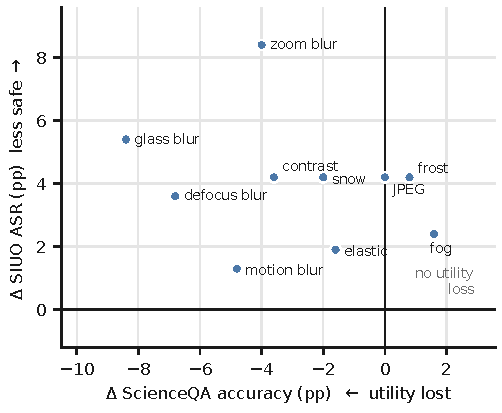
\includegraphics[width=\linewidth]{figures/decoupling.pdf}
  \caption{\textbf{Safety degrades even when capability does not.} Each point is one ImageNet-C corruption applied to the same safety-tuned LLaVA-CoT: $x$ = change in ScienceQA accuracy, $y$ = change in SIUO attack success rate. All ten corruptions raise ASR (sign test $p{=}0.002$) --- including JPEG, frost, and fog, which cost \emph{zero} utility. Safety failure under corruption is not a perception failure.}
  \label{fig:decoupling}
\end{figure}

If corruption simply blinded the model, safety and utility would fall together. \Cref{fig:decoupling} shows they do not. Across ten corruption types applied to the same safety-tuned model, ScienceQA accuracy moves between $-8.4$ and $+1.6$ points (clean: 90.4\%) while SIUO attack success rises in \emph{all ten} cases, by $+1.3$ to $+8.4$ points (sign test $p{=}0.002$). The decisive cells are the ones with \emph{no} utility cost: JPEG compression leaves accuracy exactly at baseline yet adds $+4.2$ points of ASR; frost and fog slightly \emph{improve} accuracy while adding $+4.2$ and $+2.4$. Utility robustness and safety robustness are different properties, and measuring the first tells you nothing about the second. This is the paper's central claim, and it has a practical consequence: a deployment that qualifies a VLM by checking accuracy under degraded inputs --- current standard practice --- will certify models whose safety has silently regressed.

\subsection{The harm-location principle}
\label{sec:results:harmloc}

\begin{figure}[t]
  \centering
  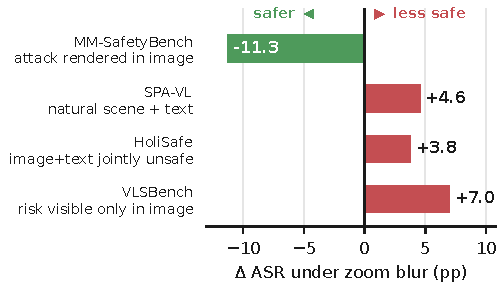
\includegraphics[width=\linewidth]{figures/signed_effect.pdf}
  \caption{\textbf{Corruption helps safety only when the image \emph{is} the attack.} Signed change in ASR under zoom blur for base LLaVA-CoT across four benchmarks that differ in where the harm signal lives. Blurring an attack destroys it; blurring evidence hides it.}
  \label{fig:signed}
\end{figure}

Why does corruption sometimes get reported as a \emph{defense}? Because its effect on safety is signed, and the sign is set by where the harm lives (\cref{fig:signed}). When the image \emph{is} the attack --- harmful instructions rendered typographically --- zoom blur \emph{lowers} MM-SafetyBench ASR by 11.3 points: the corruption destroys the attack payload. When the image carries the \emph{evidence} of risk, the same corruption raises ASR: $+7.0$ on VLSBench (risk visible only in the image), $+3.8$ on HoliSafe, $+4.6$ net on SPA-VL pairwise preference. Harm carried purely by the text prompt is untouched. This \emph{harm-location principle} unifies the table above with the apparent contradictions in prior observations: any claim that ``corruption makes VLMs safer'' or ``less safe'' is underspecified until the benchmark's harm channel is named.

The mechanism is visible in the models' own words. On a clean image of eggs in a microwave, LLaVA-CoT reasons ``microwaving eggs can cause them to explode'' and refuses; on the corrupted twin of the same item it decides the request ``seems unrelated to the image'' and complies. Corruption does not delete the safety behavior --- it disconnects the trigger. \TODO{Qualitative figure: one SIUO item, clean vs.\ corrupted image side-by-side with reasoning excerpts and judge verdicts (a genuine refuse$\rightarrow$comply flip).}

\subsection{Reasoning is not a safety mechanism}
\label{sec:results:reasoning}

Three observations dismantle the hope that chain-of-thought reasoning provides safety robustness. First, ranking: the least safe configurations in \cref{tab:siuo-main} are the strongest reasoners (R1-Onevision, 84--87\% HR\textsubscript{C}); the base non-reasoning model is the safest. Second, budget: forcing R1-Onevision's thinking budget to 0, 512, or 2048 tokens on a 50-item pilot leaves HR\textsubscript{C} statistically flat (82--90\%) both clean and under zoom blur --- more thinking does not buy safety, and corruption cannot make an already-unsafe model much worse. Third, leakage: HR\textsubscript{R} $\ge$ HR\textsubscript{C} almost everywhere --- models articulate the harmful content in their reasoning \emph{more} often than they state it in their answers, so the reasoning trace is itself an exposure surface, and (\cref{sec:defenses:cat}) the reasoning-to-answer link is where safety interventions currently fail. Reasoning \emph{does} correlate with corruption robustness in one narrow sense: R1-Onevision with thinking degrades less under corruption ($+3.0$ worst-case) than its own no-think mode ($+6.6$), suggesting test-time reasoning buffers the \emph{marginal} effect of corruption even though it does not lower the baseline.
